\begin{center}
{\LARGE DeepSeek-V4：\par}
\vspace{0.4em}
{\Large 迈向高效的百万 Token 上下文智能\par}
\vspace{0.8em}
DeepSeek-AI research@deepseek.com
\end{center}

\section*{摘要}
\addcontentsline{toc}{section}{摘要}

我们发布了 DeepSeek-V4 系列的预览版本，其中包括两款强大的混合专家（MoE）语言模型：拥有 1.6T 参数（49B 激活）的 DeepSeek-V4-Pro，以及拥有 284B 参数（13B 激活）的 DeepSeek-V4-Flash；二者都支持一百万 Token 的上下文长度。DeepSeek-V4 系列在架构与优化方面包含若干关键升级：（1）将压缩稀疏注意力（CSA）与重度压缩注意力（HCA）结合的混合注意力架构，以提升长上下文效率；（2）增强传统残差连接的流形约束超连接（mHC）；（3）用于更快收敛和更高训练稳定性的 Muon 优化器。我们在超过 32T 的多样化高质量 Token 上对两个模型进行了预训练，随后采用全面的后训练流水线来释放并进一步增强其能力。DeepSeek-V4-Pro-Max 作为 DeepSeek-V4-Pro 的最高推理力度模式，重新定义了开源模型的最新水平，在核心任务上超越了其前代。同时，DeepSeek-V4 系列在长上下文场景下也极为高效。在一百万 Token 的上下文设定中，相比 DeepSeek-V3.2，DeepSeek-V4-Pro 的单 Token 推理 FLOPs 仅为其 \(27\%\)，KV 缓存仅为其 \(10\%\)。这使我们能够常态化支持一百万 Token 上下文，从而让长时程任务和进一步的测试时扩展更加可行。模型检查点可在 \url{https://huggingface.co/collections/deepseek-ai/deepseek-v4} 获取。

\pandocbounded{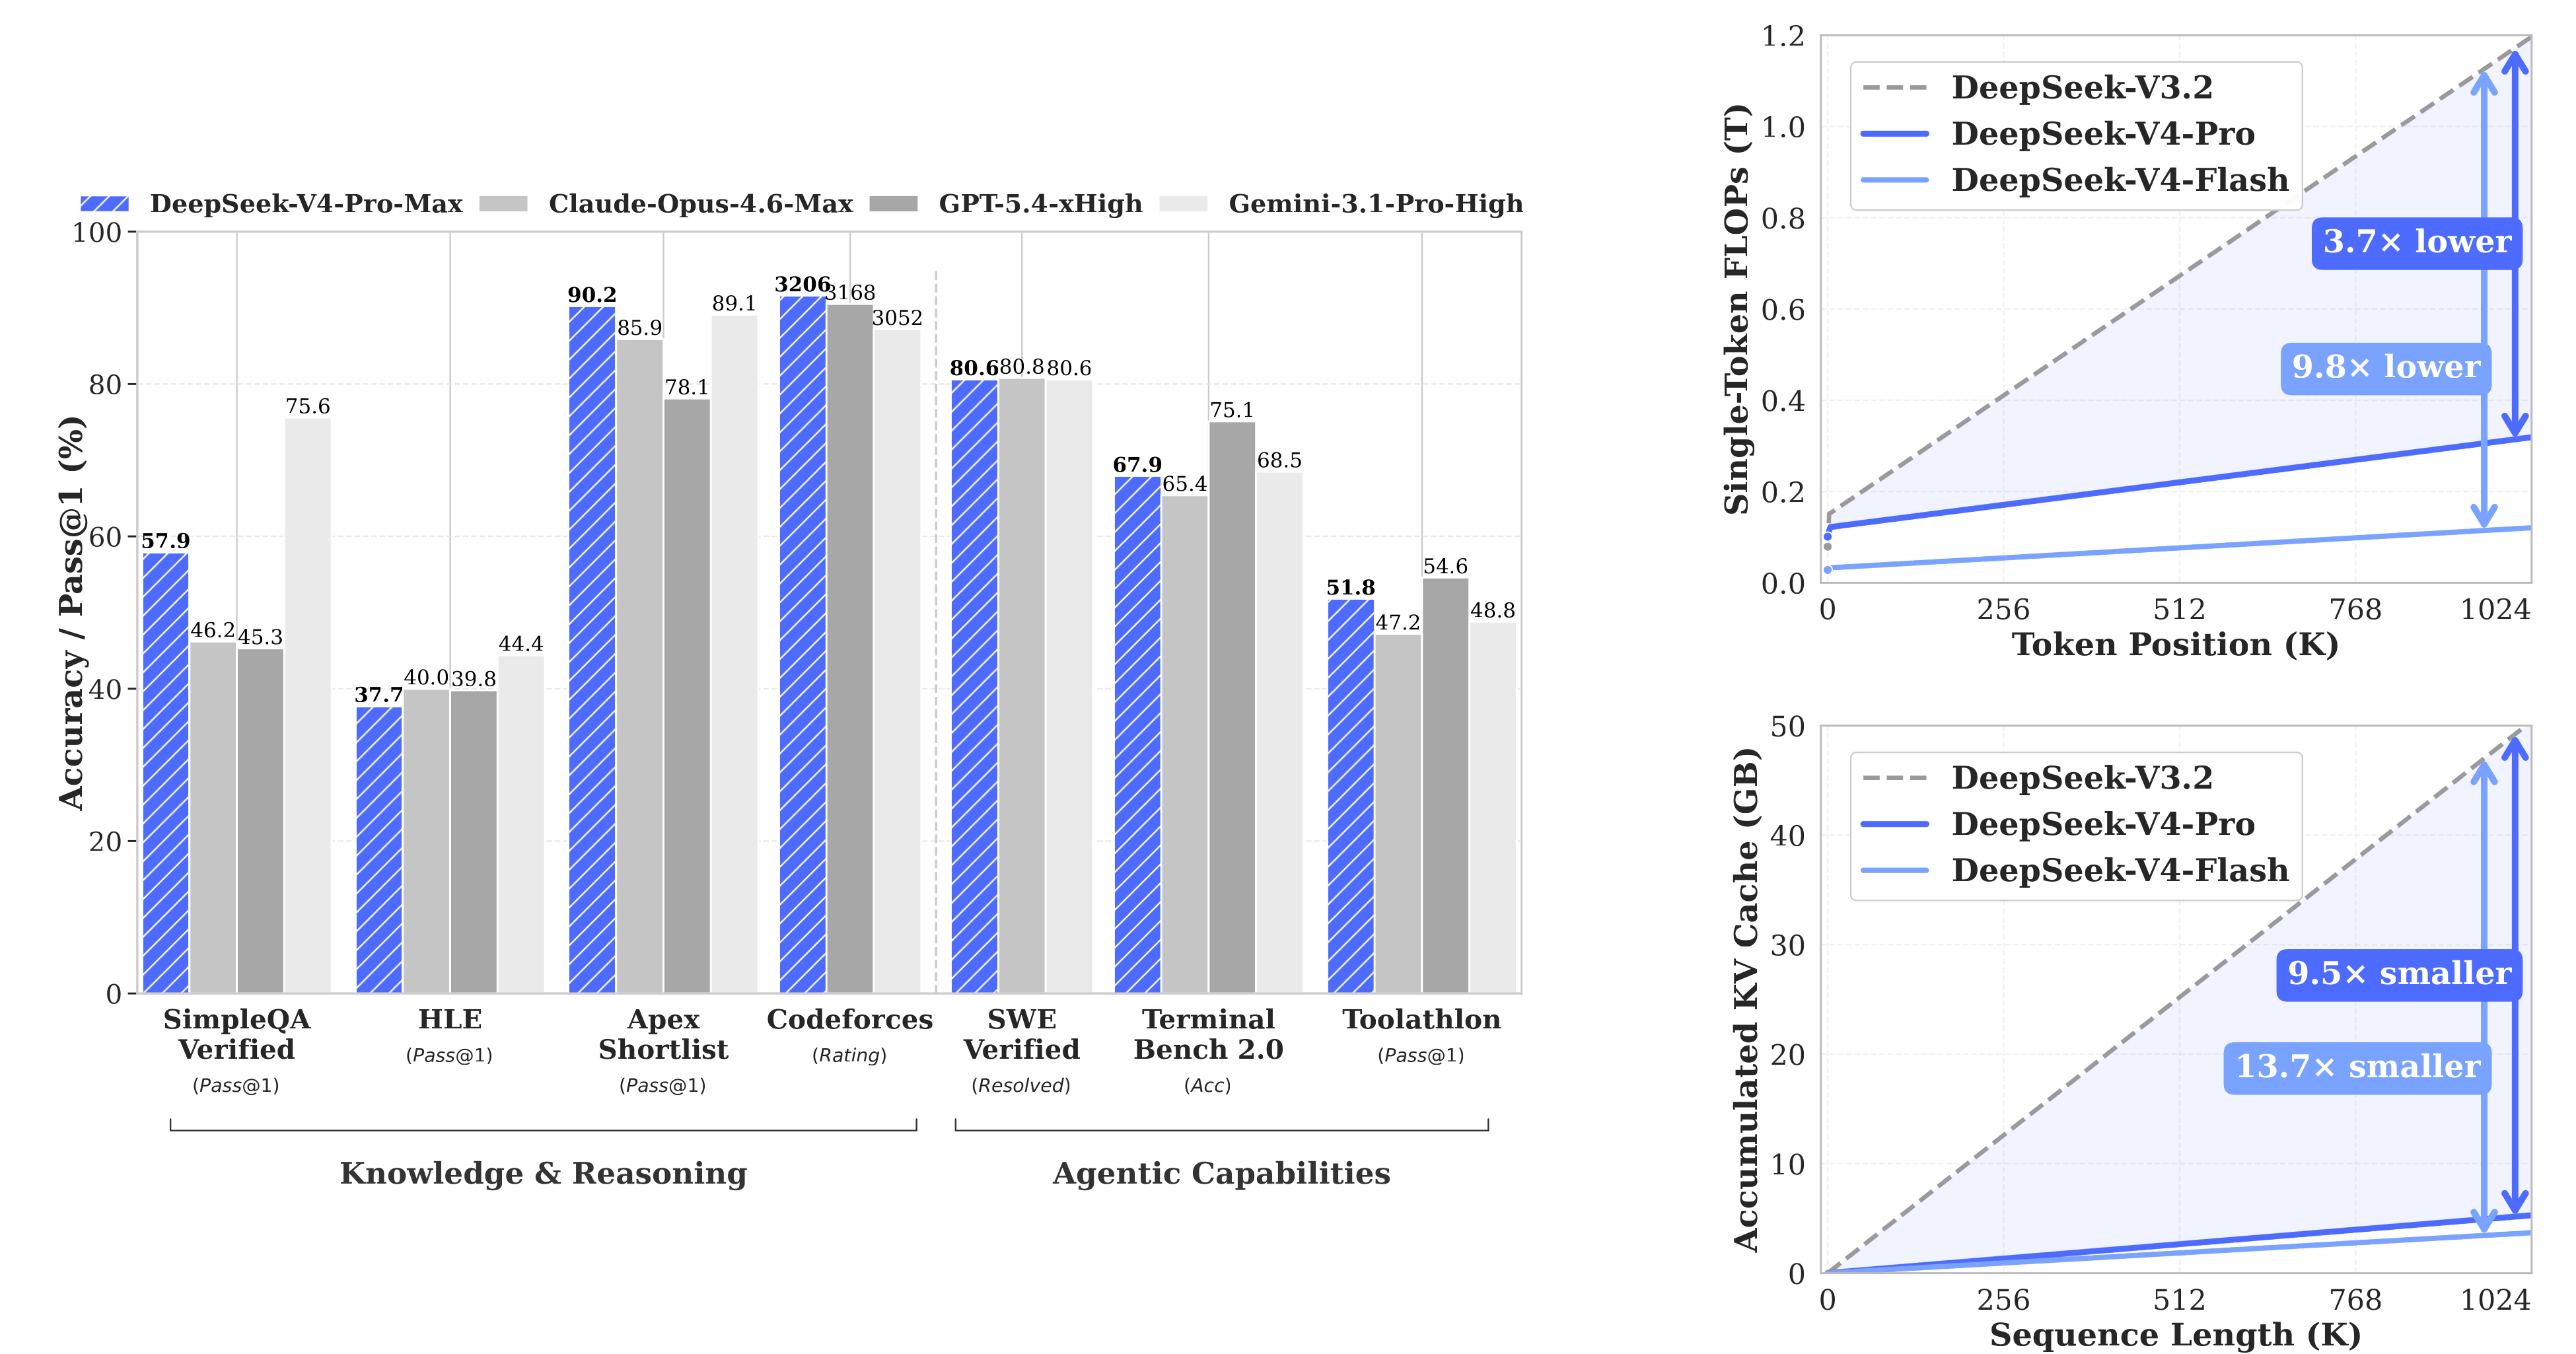
\includegraphics[keepaspectratio,alt={image}]{images_hi/Figure1_hi.png}}

图 1 \textbar{} 左：DeepSeek-V4-Pro-Max 与其对比模型的基准性能。右：DeepSeek-V4 系列与 DeepSeek-V3.2 的推理 FLOPs 与 KV 缓存大小。

\tableofcontents
\clearpage
